\documentclass{../../../oss-ap12ibhl}

\begin{document}
\genheader
\gentitle{7}{HARMONIC MOTION}

\begin{questions}

  \question A \SI{.40}{\kilo\gram} mass hangs on a spring with a spring
  constant of \SI{12}{\newton\per\metre}. The system oscillates with a constant
  amplitude of \SI{12}{\centi\metre}. What is the maximum acceleration of the
  system?
  \begin{choices}
    \choice\SI{.62}{\metre\per\second\squared}
    \choice\SI{1.4}{\metre\per\second\squared}
    \choice\SI{1.6}{\metre\per\second\squared}
    \choice\SI{3.6}{\metre\per\second\squared}
    \choice\SI{9.8}{\metre\per\second\squared}
  \end{choices}

  \question A mass is attached to a spring and allowed to oscillate vertically.
  Which of the following would NOT change the period of the oscillation?
  \begin{choices}
    \choice Double the mass and double the spring constant
    \choice Double the amplitude of vibration and double the mass
    \choice Double the gravitational field strength and double the mass
    \choice Double the gravitational field strength and double the spring
    constant
    \choice Double the gravitational field strength and quadruple the mass
  \end{choices}
    
  \question The Moon is approximately \SI{384000}{\kilo\metre} from the Earth.
  The Moon revolves around the Earth once every 27.3 days. What is the frequency
  of the Moon's motion?
  \begin{choices}
    \choice \SI{14100}{\kilo\metre} each day
    \choice 0.0366 revolution each day
    \choice 27.3 revolution each day
    \choice 655 hours for each revolution
    \choice 27.3 days for each revolution
  \end{choices}

  \question A mass is suspended from a spring and allowed to oscillate freely.
  When the amplitude of vibration is doubled, what happens to frequency of
  vibration?
  \begin{choices}
    \choice It quadruples.
    \choice It doubles.
    \choice It stays the same.
    \choice It reduces to one-half of what it was.
    \choice It reduces to one-fourth of what it was.
  \end{choices}
    
  \question A bell is rung when the dangling clapper within it makes contact
  with the bell. A poorly designed bell has a clapper that swings with the same
  period as the bell. How can this design be improved?
  \begin{choices}
    \choice Use a clapper with a smaller mass on the end so it is out of period
    with the bell.
    \choice Use a clapper with a bigger mass on the end so it is out of period
    with the bell.
    \choice Force the bell to swing with greater amplitude.
    \choice Use a longer clapper so it is out of period with the bell.
    \choice Increase the mass of the bell so it makes better contact with the
    clapper.
  \end{choices}

  \question Which choice below best explains why a pendulum does not oscillate
  in zero gravity?
  \begin{choices}
    \choice The pendulum has no mass in zero gravity.
    \choice A pendulum requires gravity to create the restoring force.
    \choice The pendulum is in orbit and considered weightless.
    \choice The pendulum would be too far from the Earth to work properly.
    \choice The pendulum must have an oscillating tension in the string to
    function properly.
  \end{choices}
    
  \question A refrigerator compressor that weighs 8 kg is fixed to three
  separate springs on the refrigerator frame. Each has a spring constant of
  \SI{0.01}{\newton\per\metre}. What is the natural frequency of the system?
  \begin{choices}
    \choice 0.01 cycle/s
    \choice 0.03 cycle/s
    \choice 0.8 cycle/s
    \choice 103 cycles/s
    \choice 0.003 cycle/s
  \end{choices}
  
  \question A pendulum on the surface of the Moon has a period of 1.0 s. If the
  length of the pendulum is quadrupled, what is the value of the new period?
  \begin{choices}
    \choice 0.25 s
    \choice 0.50 s
    \choice 1.0 s
    \choice 2.0 s
    \choice 4.0 s
  \end{choices}
    
  \question A \SI{2.}{\metre} pendulum on a particular planet has a period of
  \SI{4.6}{\second}. What is the gravitational field strength on that planet?
  \begin{choices}
    \choice\SI{1.6}{\newton\per\kilo\gram}
    \choice\SI{3.7}{\newton\per\kilo\gram}
    \choice\SI{4.9}{\newton\per\kilo\gram}
    \choice\SI{9.8}{\newton\per\kilo\gram}
    \choice\SI{25}{\newton\per\kilo\gram}
  \end{choices}

  \question The displacement (in centimeters) of the vibrating cone of a large
  loudspeaker is represented by the equation $\Delta x=2.0\cos(150t)$, where
  $t$ is the time in seconds. What distance does the tip of the cone move in
  half a period?
  \begin{choices}
    \choice 0.007 cm
    \choice 1.0 cm
    \choice 2.0 cm
    \choice 4.0 cm
    \choice 150 cm
  \end{choices}
  \newpage
  
  \question Which choice below best explains why a pendulum does not oscillate
  in zero gravity?
  \begin{choices}
    \choice The pendulum has no mass in zero gravity.
    \choice A pendulum requires gravity to create the restoring force.
    \choice The pendulum is in orbit and considered weightless.
    \choice The pendulum would be too far from the Earth to work properly.
    \choice The pendulum must have an oscillating tension in the string to
    function properly.
  \end{choices}

  \question Some large oil tankers have an antiroll water tank inside the hull
  that matches the resonant frequency of the ship’s hull. When ocean waves hit
  the ship at the resonant frequency, how does the water tank prevent the ship
  from capsizing in the waves?
  \begin{choices}
    \choice The energy of the waves is used by the water in the tank.
    \choice The waves enter the tank and are dampened.
    \choice The water tank is \ang{180} out of phase with the ship's hull.
    \choice The water tank is \ang{90} out of phase with the ship's hull.
    \choice The water in the tank is in phase with the ship's hull.
  \end{choices}
    
  \question The graph below shows the displacement versus time for an object.
  Which equation best describes its displacement in meters?
  \cpic{.45}{d-t}
  \begin{choices}
    \choice $\Delta x=20\cos(0.5t)$
    \choice $\Delta x=10\cos(2t)$
    \choice $\Delta x=10\cos(\pi t)$
    \choice $\Delta x=20\cos(2t)$
    \choice $\Delta x=20\sin(\pi t)$
  \end{choices}
    
  \question The Moon has a gravitational field strength that is approximately
  one-sixth of the field on the Earth. What is the ratio between the period
  of a pendulum on the Moon and the period of an identical pendulum on the
  Earth?
  \begin{choices}
    \choice 6
    \choice $\sqrt{6}$
    \choice $\dfrac16$
    \choice $\dfrac1{\sqrt6}$
    \choice 1
  \end{choices}

  \question Which of the following best represent periodic motion?
  \begin{choices}
    \choice A skydiver who has reached terminal velocity
    \choice The Moon in orbit about the Earth
    \choice A car driving to each state in the United States
    \choice A cart pushed up a frictionless incline plane
    %\choice A pendulum swinging over a 30-min time span.
    \choice A rubber ball bouncing on the floor over 30 seconds.
  \end{choices}
    
  \question Which of the following significantly affect the period of a simple
  pendulum?
  \begin{choices}
    \choice The length of the pendulum
    \choice The mass of the pendulum bob
    \choice The amplitude of swing
    %\choice The gravitational field strength
    \choice The shape of the mass
    \choice The thickness of the string
  \end{choices}

  \question A particle oscillates with simple harmonic motion with no damping.
  Which one of the following statements about the acceleration of the
  oscillating particle is true?
  \begin{choices}
    \choice It has a value of \SI{9.8}{\metre\per\second\squared} when the
    oscillation is vertical.
    \choice It is zero when the speed is the minimum.
    \choice It is proportional to the frequency.
    \choice It is zero throughout the oscillation.
    \choice It is zero when the speed is the maximum.
  \end{choices}
  \newpage
  
  \uplevel{
    \textbf{Questions \ref{one}--\ref{four}} are based on the figure below of a
    mass-spring system. Assume the mass is pulled back to position +A and
    released, and it slides back and forth without friction.
    \cpic{.4}{springs}
  }
  
  \question When the mass reaches position $-A$, what can be said about its
  speed?
  \label{one}
  \begin{choices}
    \choice It is a minimum.
    \choice It is a maximum.
    \choice It is zero.
    \choice It is decreasing.
    \choice It is increasing.
  \end{choices}
  
  \question When the mass reaches position 0, what can be said about its speed?
  \begin{choices}
    \choice It is a minimum.
    \choice It is a maximum.
    \choice It is zero.
    \choice It is decreasing.
    \choice It is increasing.
  \end{choices}
    
  \question At what position does the mass have the greatest acceleration?
  \begin{choices}
    \choice $-A$
    \choice $-A/2$
    \choice 0
    \choice $+A/2$
    \choice $+A$
  \end{choices}
    
  \question The mass is released from the $-A$ position at time $t=0$, and it
  oscillates with period $T$, measured in seconds. Which equation best
  represents the displacement?
  \label{four}
  \begin{choices}
    \choice $\Delta x = -A\cos\left(\dfrac{T}{2\pi}t\right)$
    \choice $\Delta x = -(A/2)\cos(2\pi T t)$
    \choice $\Delta x = -A\cos\left(\dfrac{2\pi}{T}t\right)$
    \choice $\Delta x = (A/2)\cos(T t)$
    \choice $\Delta x = A\cos\left(\dfrac{2\pi}{T}t\right)$
  \end{choices}
  \newpage
%
%\genfreetitle{1}{SIMPLE HARMONIC MOTION}{4}
%
%\genfreedirections
%
  % TAKEN FROM 2018 AP PHYSICS 1 FREE-RESPONSE QUESTION #5
  \uplevel{
    \cpic{.5}{blocks}
  }
  \question Block $P$ of mass $m$ is on a horizontal, frictionless surface and
  is attached to a spring with spring constant $k$. The block is oscillating
  with period $T_P$ and amplitude $A_P$ about the spring's equilibrium position
  $x_0$. A second block $Q$ of mass $2m$ is then dropped from rest and lands on
  block $P$ at the instant it passes through the equilibrium position, as shown
  above. Block $Q$ immediately sticks to the top of block $P$, and the
  two-block system oscillates with period $T_{PQ}$ and amplitude $A_{PQ}$.
  \begin{parts}
    \part Determine the numerical value of the ratio $T_{PQ}/T_P$.
    
  \part How does the amplitude of oscillation $A_{PQ}$ of the two-block system
    compare with the original amplitude $A_P$ of block $P$ alone?

    \vspace{.1in}
    \underline{\hspace{.3in}} $A_{PQ}<A_{P}$\hspace{.25in}
    \underline{\hspace{.3in}} $A_{PQ}=A_{P}$\hspace{.25in}
    \underline{\hspace{.3in}} $A_{PQ}>A_{P}$

    \vspace{.2in}In a clear, coherent paragraph-length response that may also
    contain diagrams and/or equations, explain your reasoning.
  \end{parts}
  \newpage

  \question In heavy seas, the bow of a battle ship undergoes a simple harmonic
  vertical pitching motion with a period of \SI{8.}{\second} and an amplitude
  of \SI{2.}{\metre}.
  \begin{parts}
    \part What is the maximum vertical velocity of the battle ship's bow?
    \part What is its maximum acceleration?
    \part An \SI{80}{\kilo\gram} sailor is standing on the scale in the bunk
    room in the bow. What are the maximum and minimum reading on the scale in
    newtons?
  \end{parts}
  \newpage
  
  \question Show that for the situations in the figures below, the object of
  mass $m$ oscillates with a frequency of $\omega=\sqrt{\dfrac{k_\text{eff}}m}$
  where $k_\text{eff}$ is given by (a) $k_\text{eff}=k_1+k_2$ and (b)
  $\dfrac1{k_\text{eff}}=\frac1{k_1}+\frac1{k_2}$. Hint: find the net force on
  the mass and write $F=-k_\text{eff}x$. Note that in (b), the springs stretch
  by different amounts, the sum of which is $x$.
  
  (a)\hspace{5pt}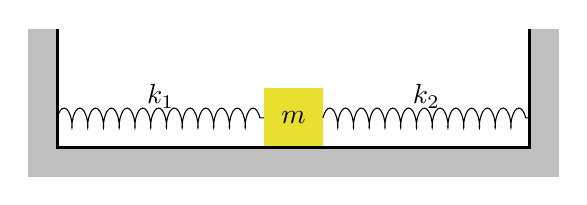
\begin{tikzpicture}[scale=.5]
    \fill[gray!50](0,0) rectangle(12,-.75);
    \fill[gray!50](-.75,-.75) rectangle(0,3);
    \fill[gray!50](12,-.75) rectangle(12.75,3);
    \fill[yellow!80!gray](5.25,0) rectangle(6.75,1.5) node[midway,black]{$m$};
    \draw[decoration={aspect=0.3,segment length=2mm, amplitude=1.25mm, coil},
      decorate] (0,.75)--(5.25,.75) node[midway,above]{$k_1$};
    \draw[decoration={aspect=0.3,segment length=2mm, amplitude=1.25mm, coil},
      decorate] (6.75,.75)--(12,.75) node[midway,above]{$k_2$};
    \draw[very thick](0,3)--(0,0)--(12,0)--(12,3);
  \end{tikzpicture}
  
  (b)\hspace{5pt}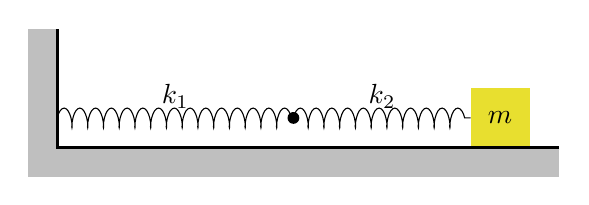
\begin{tikzpicture}[scale=.5]
    \fill[gray!50](0,0) rectangle(12.75,-.75);
    \fill[gray!50](-.75,-.75) rectangle(0,3);
    \fill[yellow!80!gray](10.5,0) rectangle(12,1.5) node[midway,black]{$m$};
    \draw[decoration={aspect=0.3,segment length=2mm, amplitude=1.25mm, coil},
      decorate] (0,.75)--(6,.75) node[midway,above]{$k_1$};
    \draw[decoration={aspect=0.3,segment length=2mm, amplitude=1.25mm, coil},
      decorate] (6,.75)--(10.5,.75) node[midway,above]{$k_2$};
    \fill[black](6,.75) circle(.15);
    \draw[very thick](0,3)--(0,0)--(12.75,0);
  \end{tikzpicture}
  \newpage
  
  \question A simple pendulum of length $L$ is released from rest from an angle
  of $\theta_0$.
  \begin{parts}
    \part Assuming the motion of the pendulum to be simple harmonic motion, find
    its speed as it passes through $\theta=0$.
    \part Using the conservation of energy, find this speed exactly.
    \part Show that your results for (a) and (b) are the same when $\theta_0$ is
    small.
    \part Find the difference in your results for $\theta_0=\SI{.20}{rad}$ and
    $L=\SI1{\metre}$.
  \end{parts}
\end{questions}
\end{document}
